\section{Discussion and Results}
\label{chap:Discussion and Results}

\subsection{Handling the raw data and choosing a security}
\label{chap:Handling the raw data and choosing a security}

\quad Our raw data came from B3 Brazilian's stock exchange, which can be download freely from \href{http://www.b3.com.br/pt_br/market-data-e-indices/servicos-de-dados/market-data/cotacoes/cotacoes/}{its website}. The files contain all negotiations (historical series of data) for all securities from a trading section (day). We have downloaded the files containing the data-series from 22.06.2020 to 04.12.2020, and the chosen security that our studies will focus on will be PETR4. For that, a python function called get\_instrument() in the \href{https://github.com/fabiorodp/UiO-FYS-STK4155/tree/master/Project3/package/read_data.py}{Project3/package/read\_data.py} file does the job of extracting all negotiations for PETR4.\\

It is essential to state that PETR4 is the biggest specialized company in Brazil's oil, natural gas, and energy industry. Besides, in the B3 market, this stock has one of the highest liquidity flow that guarantee us to avoid higher price gaps, slippage, or any other trading issues. These reasons justify our choice for PETR4, but any additional security can perform the following experiments.

\subsection{Engineering the features and deciding the prediction's targets}
\label{chap:Engineering the features and deciding the prediction's targets}

\quad Most of the studies using ANN for time series forecasting uses input data holding the stock daily (OLHC) opening, lowest, highest, and closing prices \hyperref[Bib:Leonardo C. Martinez, Diego N. da Hora, Joao R. de M. Palotti, Wagner Meira Jr. and Gisele L. Pappa]{[5]}\hyperref[Bib:Van-Dai Ta, Chuan-Ming Liu, Direselign Addis Tadesse]{[6]}. The input may include many other \hyperref[chap:Technical Analysis]{technical analysis (TA)} or fundamental analysis (FA) indicators.\\

As this report considers short-term trading structures, there is no reason to use fundamentalists' indicators published quarterly. However, technical indicators are very relevant and useful to bring more information to our ANN's models. Hence, as introduced in the theory section of this work, we will use three technical tools, such that, \hyperref[chap:Simple Moving Average (SMA)]{Simple Moving Average (SMA)}, \hyperref[chap:Exponential Moving Average (EMA)]{Exponential Moving Average (EMA)}, and \hyperref[chap:Bollinger Bands (BB)]{Bollinger Bands (BBs)}.\\

Therefore, the 16 variables/features used as input to RNN and LSTM are described in the following table:

\begin{table}[H]
\centering
\begin{tabular}{ |p{1cm}||p{11cm}|  }
\hline
\multicolumn{2}{|c|}{Features for training data} \\
\hline
\centering
Qtd & Description\\
\hline
\centering
4   & The opening, lowest, highest, closing prices and volume (OLHCV);\\
\centering
9   & The upper, middle and lower BBs for 5, 10 and 20 periods;\\
\centering
3   & The EMAs for 5, 10 and 20 periods.\\
\hline
\end{tabular}
\label{table:TrainingFeatures}
\caption{Variables/features used as input to RNN and LSTM models.}
\end{table}

%\bigskip

Remark that these features test the ability of the RNN and LSTM to learn from previous information of the time series data. Besides, these features were chosen according to the author's trading practices, but it could have been chosen in any other preferable periods. As a future research objective, it would be a relevant idea to study the effect of several indicators in the learning and the appropriate amount of historical data that should be considered.\\

Regarding the prediction's targets, we want to design a valuable tool for algorithm tradings and decision-making processes. The idea is to predict the highest and lowest of the next trading section (next day). This information would bring a rouge advance and benefit for day-traders because they will start the day already knowing the probable highest and lowest and, consequently, avoid trading operations in the wrong direction against the oversold (lowest of the day) overbought (highest of the day) areas.

\subsection{Time series Cross-Validation}
\label{chap:Time series Cross-Validation}

\quad The Machine Learning system, in general, learns the data's structure so that we can predict the future. When we fit and train the learning algorithm, it does not surprise the spectacular results that can be found. Still, it typically has zero forecasting power if not tested with unseen data \hyperref[Bib:Lopez de Prado]{[4][p. 131]}. Therefore, one solution is to perform Cross-Validation (CV) splits, where we separate the entire data on training and testing sets.\\

Regarding time-series data, the typical CV, which handles independent identically distributed (IID) sets, fails in its proposes. Indeed, we are dealing with ordered, recurrent, and serially-correlated data, which can not be split into unordered blocks or even shuffled. Besides, it is also common to have leakage \hyperref[Bib:Lopez de Prado]{[4][p. 131]} when pieces of information from the training set also arise in the testing sets. One widespread example of leakage is when one wants to predict a period's closing price giving the highest and lowest of the same time step. The ideal in this scenario is to provide the highest and lowest of the previous time step. Thinking on leakage, Professor Marcos Lopes de Prado elaborated a policy to reduce the likelihood of leakage, \textit{ipsis verbis} \hyperref[Bib:Lopez de Prado]{[4][p. 132]}:\\

\noindent \textit{\textbf{1st.} Drop from the training set any observation $i$ where $Y_i$ is a function of information used to determine $Y_j$, and $j$ belongs to the testing set.}\\

\qquad \textit{\textbf{(a)} For examples, $Y_i$ and $Y_j$ should not span overlapping periods.}\\

\noindent \textit{\textbf{2nd.} Avoid over-fitting the classifier. In this way, even if some leakage occurs, the classifier will not be able to profit from it. Use:}\\

\qquad \textit{\textbf{(a)} Early stopping of the base estimators;}\\

\qquad \textit{\textbf{(b)} Bagging of classifiers, while controlling for oversampling on redundant examples, so that the individual classifiers are as diverse as possible.}\\

\qquad \qquad \textit{\textbf{(b.i)} Set max\_samples to the average uniqueness.}\\

\qquad \qquad \textit{\textbf{(b.ii)} Apply sequential bootstrap.}\\

In this project, we have followed Prado's policies for avoiding leakages.\\

For the CV technique, we have used the proposed methodology given by \hyperref[Bib:Hyndman, R.J., and Athanasopoulos, G.]{[9]}[\href{https://otexts.com/fpp2/}{Ch.3.4}], which describes a procedure for testing unseen data with series of test sets containing a single observation, and the corresponding training set consists of rolled samples that occurred before. The diagram that illustrates the series of training and testing sets follows \hyperref[Bib:Hyndman, R.J., and Athanasopoulos, G.]{[9][Ch.3.4]}:

\begin{figure}[H]
\label{fig:CV}
\centering
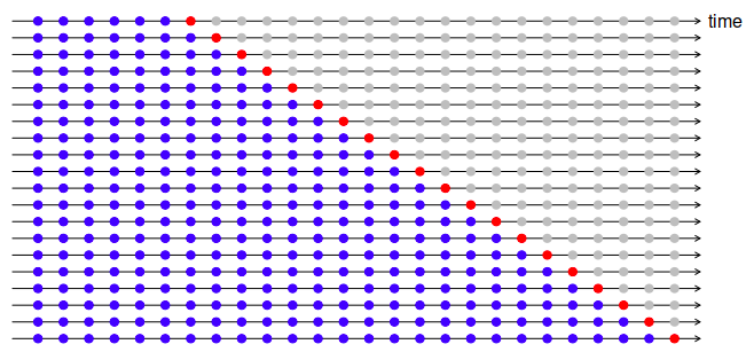
\includegraphics[height=4cm]{CV}
\caption{Time series CV using \textit{"evaluation on a rolling forecasting origin"}\hyperref[Bib:Hyndman, R.J., and Athanasopoulos, G.]{[9][Ch.3.4]}}
\end{figure}

The accuracy of the predictions will be calculated by averaging over the Mean Squared Error (MSE) and Mean Absolute Error (MAE) resulted from all training and validations. This method is called \textit{"evaluation on a rolling forecasting origin"} by the authors \hyperref[Bib:Hyndman, R.J., and Athanasopoulos, G.]{[9][Ch.3.4]} because of the training sets based on rolls ahead in time.\\

Our script called \href{https://github.com/fabiorodp/UiO-FYS-STK4155/tree/master/Project3/package/studies.py}{studies.py} in \href{https://github.com/fabiorodp/UiO-FYS-STK4155/tree/master/Project3/package/}{Project3/package/} directory performs a Time series Cross-Validation with parameter combination of Units and Epochs. The beginning's rolling value for training is defined by default as 60-time steps, which means that our ANN model will start the training with the first 60-days of data, and then it validates the 61's day and measure the testing metrics. The CV algorithm keeps doing the same procedure for the next steps, training 61-days and validating the 62's day, until all data have been gone. In the end, the average testing metrics are returned for an assessment of the best model and parameters.

\subsection{Training RNN model and optimizing hyper-parameters}
\label{chap:Training RNN model and optimizing hyper-parameters}

\quad This section will feed and fit a \href{https://www.tensorflow.org/api_docs/python/tf/keras/layers/SimpleRNN}{SimpleRNN} model from Keras with our features and targets using the \hyperref[chap:Time series Cross-Validation]{\textit{Time Series Cross-Validation}} discussed before. A combination of parameters is applied with different numbers for units, several activation functions and various numbers of hidden-layers for epoch equals 50 and mini batch equals 1 avoiding costly computations, as follow:

\begin{table}[H]
\centering
\begin{tabular}{ |p{2.5cm}||p{7cm}|  }
\hline
\multicolumn{2}{|c|}{Hyper-parameters} \\
\hline
Name & Values\\
\hline
Act. Functions & Sigmoid, Tanh, ReLu;\\
Hidden-layers & For Sigmoid and Tanh: 1, 2; For ReLu: 2, 3;\\
Units & 50, 100, 150, 200, 400, 600, 800, 1000, 1200;\\
Epoch & 50;\\
Mini-batch & 1;\\
Loss-Function & Mean Squared Error (MSE);\\
\hline
\end{tabular}
\label{table:Hyper-parameters for SimpleRNN}
\caption{Hyper-parameters used for optimization of the SimpleRNN model.}
\end{table}

Our aim here is to find the most promising model (lowest testing MSE and MAE) with the most efficient parameters (lowest number of units as function of hidden layers and activation function). For that, we need to investigate which parameter (activation function, hidden-layers, and units) combination is the best. Further, the experiments will be based on the loss-curve, the number of epochs and any other possible way of optimization.\\

The test file \href{https://github.com/fabiorodp/UiO-FYS-STK4155/tree/master/Project3/RNN.py}{RNN.py} stored in our GitHub repository replicates all the following results in the next sub-sections.

\subsubsection{Predicting the highest price of the next day using RNN}
\label{chap:Predicting the highest price of the next day using RNN}

\quad We start experimenting the input data presented in \hyperref[table:TrainingFeatures]{Table 1} on the SimpleRNN model with various combinations of parameters as delineated in \hyperref[table:Hyper-parameters for SimpleRNN]{Table 2}. The goal is to optimize the SimpleRNN model for predicting the highest price of the next day with the most promising and effective parameters as explained in \hyperref[chap:Training RNN model and optimizing hyper-parameters]{\textit{Taining RNN model and optimizing hyper-parameters}} section.\\

Starting with Sigmoid's activation function and hidden-layers 1 and 2, the results follow:

\begin{table}[H]
\centering
\resizebox{\textwidth}{110}{
\begin{tabular}{ |c|c|c|c|c|c|c| }
\hline
\textbf{Act. Funct.} & \textbf{H-layers} & \textbf{Units} & \textbf{Train MSE} & \textbf{Test MSE} & \textbf{Train MAE} & \textbf{Test MAE}\\
\hline
Sigmoid & 1 & 15 & 2.78 &  7.54 &  1.43 &  2.37\\
Sigmoid & 1 & 50 & 2.06 &	7.93 &	1.25 &	2.45\\
Sigmoid & 1 & 100 & 1.95 &	7.92 &	1.16 &	2.33\\
Sigmoid & 1 & 150 & 1.76 &	7.57 &	1.04 &	2.21\\
Sigmoid & 1 & 200 & 1.48 &	6.61 &	0.89 &	2.02\\
Sigmoid & 1 & 400 & 0.73 &	2.77 &	0.57 &	1.33\\
Sigmoid & 1 & 600 & 0.51 &	1.33 &	0.47 &	0.88\\
Sigmoid & 1 & 800 & 0.42 &	0.82 &	0.42 &	0.63\\
Sigmoid & 1 & 1000 & 0.38 &	0.65 &	0.40 &	0.52\\
\rowcolor{lightgray} \textbf{Sigmoid} & \textbf{1} & \textbf{1200} & \textbf{0.37} &	\textbf{0.55} &	\textbf{0.40} &	\textbf{0.49}\\
\hline
\hline
Sigmoid & 2 & 15  &  2.08 &	7.82 &	1.27 &	2.47\\
Sigmoid & 2 & 50  &  0.54 &	1.63 &	0.50 &	0.99\\
Sigmoid & 2 & 100 &  0.40 &	0.89 &	0.42 &	0.65\\
Sigmoid & 2 & 150 &  0.41 &	0.90 &	0.42 &	0.66\\
Sigmoid & 2 & 200 &  0.42 &	0.94 &	0.43 &	0.68\\
Sigmoid & 2 & 400 &  0.43 &	0.81 &	0.43 &	0.62\\
Sigmoid & 2 & 600 &  0.37 &	0.56 &	0.40 &	0.49\\
\rowcolor{lightgray} \textbf{Sigmoid} & \textbf{2} & \textbf{800} &  \textbf{0.38} &	\textbf{0.48} &	\textbf{0.43} &	\textbf{0.45}\\
Sigmoid & 2 & 1000 & 0.44 & 0.49 &	0.47 &	0.48\\
Sigmoid & 2 & 1200 & 0.52 & 0.56 &	0.51 &	0.52\\
\hline
\end{tabular}}
\label{table:Results for RNN, Sigmoid, High}
\caption{Parameters' combinations for predicting the next day's highest price.}
\end{table}

\hyperref[table:Results for RNN, Sigmoid, High]{Table 3} shows that the Testing MSE and MAE achieve their best-validated accuracy values of 0.55 and 0.49 for one hidden-layer and 0.48 and 0.45 for two hidden-layers. Note that the metrics for one hidden-layer have not hit the lowest by 1200 units, although it might have happened if we have increased the number of units even more. However, increasing the number of units above 1200 is very costly for computations, and it would be better practice to increase the number of hidden-layers instead. Indeed, the best accuracy metrics for two hidden-layers were by 800 units where is the optimal point for the model because, above that, the metrics worsen again.\\

Next, we perform Tanh's activation function for hidden-layers 1 and 2, the outcomes go:

\begin{table}[H]
\centering
\resizebox{\textwidth}{110}{
\begin{tabular}{ |c|c|c|c|c|c|c| }
\hline
\textbf{Act. Funct.} & \textbf{H-layers} & \textbf{Units} & \textbf{Train MSE} & \textbf{Test MSE} & \textbf{Train MAE} & \textbf{Test MAE}\\
\hline
Tanh & 1 & 15 & 2.08 &	7.82 &	1.27 &	2.47\\
Tanh & 1 & 50 & 1.96 &	7.97 &	1.17 &	2.34\\
Tanh & 1 & 100 & 1.46 &	6.52 &	0.88 &	2.01\\
Tanh & 1 & 150 & 0.98 &	4.32 &	0.67 &	1.65\\
Tanh & 1 & 200 & 0.73 &	2.76 &	0.57 &	1.34\\
Tanh & 1 & 400 & 0.42 &	0.83 &	0.42 &	0.63\\
Tanh & 1 & 600 & 0.37 &	0.56 &	0.40 &	0.49\\
\rowcolor{lightgray} \textbf{Tanh} & \textbf{1} & \textbf{800} & \textbf{0.38} &	\textbf{0.48} &	\textbf{0.43} &	\textbf{0.45}\\
Tanh & 1 & 1000 & 0.44 & 0.49 &	0.47 &	0.48\\
Tanh & 1 & 1200 & 0.52 & 0.56 &	0.51 &	0.52\\
\hline
\hline
Tanh & 2 & 15 & 2.08 &	7.82 &	1.27 &	2.47\\
Tanh & 2 & 50 & 0.42 &	1.00 &	0.43 &	0.71\\
Tanh & 2 & 100 & 0.42 &	1.04 &	0.43 &	0.73\\
Tanh & 2 & 150 & 0.46 &	1.19 &	0.45 &	0.82\\
Tanh & 2 & 200 & 0.50 &	1.27 &	0.47 &	0.85\\
Tanh & 2 & 400 & 0.45 &	0.80 &	0.43 &	0.62\\
Tanh & 2 & 600 & 0.37 &	0.56 &	0.41 &	0.48\\
\rowcolor{lightgray} \textbf{Tanh} & \textbf{2} & \textbf{800} & \textbf{0.39} & \textbf{0.51} &	\textbf{0.44} &	\textbf{0.47}\\
Tanh & 2 & 1000 & 0.44 & 0.49 &	0.47 &	0.48\\
Tanh & 2 & 1200 & 0.52 & 0.56 &	0.51 &	0.52\\
\hline
\end{tabular}}
\label{table:Results for RNN, Tanh, High}
\caption{Parameters' combinations for predicting the next day's highest price.}
\end{table}

\hyperref[table:Results for RNN, Tanh, High]{Table 4} exhibits that the Testing MSE and MAE obtain their best-validated accuracy values of 0.48 and 0.45 for one hidden-layer and 0.51 and 0.47 for two hidden-layers. Remark that the optimal point happened at units equals 800 for both one or two hidden-layers. Thus, we would choose one-hidden layer as the best model because it is costly less-expensive and got slightly better metrics than two hidden-layers.\\

Finally, ReLu's activation function is run for hidden-layers 2 and 3 with the measures:

\begin{table}[H]
\centering
\resizebox{\textwidth}{110}{
\begin{tabular}{ |c|c|c|c|c|c|c| }
\hline
\textbf{Act. Funct.} & \textbf{H-layers} & \textbf{Units} & \textbf{Train MSE} & \textbf{Test MSE} & \textbf{Train MAE} & \textbf{Test MAE}\\
\hline
ReLu & 2 & 15 & 2.13 &	7.55 &	1.29 &	2.43\\
ReLu & 2 & 50 & 1.96 &	7.97 &	1.17 &	2.34\\
ReLu & 2 & 100 & 1.46 &	6.52 &	0.88 &	2.01\\
ReLu & 2 & 150 & 0.98 &	4.32 &	0.67 &	1.65\\
ReLu & 2 & 200 & 0.73 &	2.76 &	0.57 &	1.34\\
ReLu & 2 & 400 & 0.42 &	0.83 &	0.42 &	0.63\\
ReLu & 2 & 600 & 0.37 &	0.56 &	0.40 &	0.49\\
\rowcolor{lightgray} \textbf{ReLu} & \textbf{2} & \textbf{800} & \textbf{0.38} &	\textbf{0.48} &	\textbf{0.43} &	\textbf{0.45}\\
ReLu & 2 & 1000 & 0.44 & 0.49 &	0.47 &	0.48\\
ReLu & 2 & 1500 & 0.70 & 0.60 &	0.55 &	0.55\\
\hline
\hline
ReLu & 3 & 15 & 2.08 &	7.82 &	1.27 &	2.47\\
ReLu & 3 & 50 & 0.42 &	0.99 &	0.43 &	0.71\\
ReLu & 3 & 100 & 0.42 &	1.05 &	0.43 &	0.73\\
ReLu & 3 & 150 & 0.46 &	1.19 &	0.45 &	0.82\\
ReLu & 3 & 200 & 0.50 &	1.29 &	0.47 &	0.86\\
ReLu & 3 & 400 & 0.44 &	0.80 &	0.43 &	0.62\\
ReLu & 3 & 600 & 0.37 &	0.56 &	0.41 &	0.48\\
\rowcolor{lightgray} \textbf{ReLu} & \textbf{3} & \textbf{800} & \textbf{0.39} &	\textbf{0.48} &	\textbf{0.44} &	\textbf{0.45}\\
ReLu & 3 & 1000 & 0.44 & 0.49 &	0.47 &	0.48\\
ReLu & 3 & 1200 & 0.52 & 0.56 &	0.51 &	0.52\\
\hline
\end{tabular}}
\label{table:Results for RNN, ReLu, High}
\caption{Parameters' combinations for predicting the next day's highest price.}
\end{table}

\hyperref[table:Results for RNN, ReLu, High]{Table 5} reveals that the Testing MSE and MAE reach their best-validated accuracy values of 0.48 and 0.45 for two hidden-layer and 0.48 and 0.45 for three hidden-layers. Important to state that ReLu with one hidden-layer makes the computations explode to a very high value, then it was not considered in this report. On the other hand, there is no relevant difference between training ReLu with two or three hidden-layers because both got the same best-validated accuracy metrics by 800 units.\\

\subsubsection{Predicting the lowest price of the next day using RNN}
\label{chap:Predicting the lowest price of the next day using RNN}

\quad Now, we apply again the input data presented in \hyperref[table:TrainingFeatures]{Table 1} on the SimpleRNN model with various combinations of parameters as delineated in \hyperref[table:Hyper-parameters for SimpleRNN]{Table 2}. The goal is to optimize the SimpleRNN model for predicting the lowest price of the next day with the most promising and effective parameters as explained in \hyperref[chap:Training RNN model and optimizing hyper-parameters]{\textit{Taining RNN model and optimizing hyper-parameters}} section.\\

From Sigmoid's activation function and hidden-layers 1 and 2, the results follow:

\begin{table}[H]
\centering
\resizebox{\textwidth}{110}{
\begin{tabular}{ |c|c|c|c|c|c|c| }
\hline
\textbf{Act. Funct.} & \textbf{H-layers} & \textbf{Units} & \textbf{Train MSE} & \textbf{Test MSE} & \textbf{Train MAE} & \textbf{Test MAE}\\
\hline
Sigmoid & 1 & 15 & 2.47 & 7.03 & 1.36 &	2.23\\
Sigmoid & 1 & 50 & 2.12 & 7.39 & 1.26 &	2.33\\
Sigmoid & 1 & 100 & 1.95 & 7.92 & 1.16 & 2.33\\
Sigmoid & 1 & 150 & 1.76 &	7.57 &	1.04 &	2.21\\
Sigmoid & 1 & 200 & 1.48 &	6.00 &	0.91 &	1.93\\
Sigmoid & 1 & 400 & 0.73 &	2.44 &	0.59 &	1.29\\
Sigmoid & 1 & 600 & 0.49 &	0.97 &	0.47 &	0.81\\
Sigmoid & 1 & 800 & 0.40 &	0.61 &	0.42 &	0.61\\
Sigmoid & 1 & 1000 & 0.37 &	0.49 &	0.40 &	0.53\\
\rowcolor{lightgray} \textbf{Sigmoid} & \textbf{1} & \textbf{1200} & \textbf{0.36} &	\textbf{0.46} &	\textbf{0.40} &	\textbf{0.51}\\
\hline
\hline
Sigmoid & 2 & 15 & 2.15 & 7.37 & 1.28 &	2.37\\
Sigmoid & 2 & 50 & 0.54 & 1.35 & 0.50 &	0.96\\
Sigmoid & 2 & 100 & 0.39 &	0.60 &	0.42 &	0.59\\
Sigmoid & 2 & 150 & 0.39 &	0.64 &	0.43 &	0.61\\
Sigmoid & 2 & 200 & 0.40 &	0.67 &	0.43 &	0.62\\
Sigmoid & 2 & 400 & 0.42 &	0.63 &	0.42 &	0.60\\
\rowcolor{lightgray} \textbf{Sigmoid} & \textbf{2} & \textbf{600} & \textbf{0.36} &	\textbf{0.44} &	\textbf{0.40} &	\textbf{0.50}\\
Sigmoid & 2 & 800 & 0.38 &	0.42 &	0.42 &	0.51\\
Sigmoid & 2 & 1000 & 0.43 &	0.44 &	0.45 &	0.53\\
Sigmoid & 2 & 1200 & 0.48 &	0.47 &	0.50 &	0.57\\
\hline
\end{tabular}}
\label{table:Results for RNN, Sigmoid, Low}
\caption{Parameters' combinations for predicting the next day's lowest price.}
\end{table}

\hyperref[table:Results for RNN, Sigmoid, Low]{Table 6} demonstrates that the Testing MSE and MAE achieve their best-validated accuracy values of 0.46 and 0.51 for one hidden-layer and 0.44 and 0.50 for two hidden-layers. As occurred before, the metrics for one hidden-layer have not hit the lowest by 1200 units. The convergence to the minimum would happen if the number of units or number of epoch increases, but it would increase the computations' cost. In this report, we restricted these number, but for future experiments, it would be relevant to investigate these topics.\\

Now, we perform Tanh's activation function for hidden-layers 1 and 2, and the outcomes go:

\begin{table}[H]
\centering
\resizebox{\textwidth}{110}{
\begin{tabular}{ |c|c|c|c|c|c|c| }
\hline
\textbf{Act. Funct.} & \textbf{H-layers} & \textbf{Units} & \textbf{Train MSE} & \textbf{Test MSE} & \textbf{Train MAE} & \textbf{Test MAE}\\
\hline
Tanh & 1 & 15 & 2.15 &	7.37 &	1.28 &	2.37\\
Tanh & 1 & 50 & 1.99 &	7.38 &	1.18 &	2.25\\
Tanh & 1 & 100 & 1.46 &	5.87 &	0.90 &	1.92\\
Tanh & 1 & 150 & 0.98 &	3.76 &	0.69 &	1.56\\
Tanh & 1 & 200 & 0.72 &	2.30 &	0.58 &	1.25\\
Tanh & 1 & 400 & 0.40 &	0.60 &	0.42 &	0.60\\
\rowcolor{lightgray} \textbf{Tanh} & \textbf{1} & \textbf{600} & \textbf{0.36} &	\textbf{0.45} &	\textbf{0.40} &	\textbf{0.50}\\
Tanh & 1 & 800 & 0.38 &	0.42 &	0.42 &	0.51\\
Tanh & 1 & 1000 & 0.43 & 0.44 &	0.45 &	0.53\\
Tanh & 1 & 1200 & 0.48 & 0.47 &	0.50 &	0.57\\
\hline
\hline
Tanh & 2 & 15 & 2.15 &	7.37 &	1.28 &	2.37\\
Tanh & 2 & 50 & 0.40 &	0.69 &	0.43 &	0.64\\
Tanh & 2 & 100 & 0.40 &	0.77 &	0.43 &	0.67\\
Tanh & 2 & 150 & 0.46 &	0.90 &	0.45 &	0.73\\
Tanh & 2 & 200 & 0.47 &	1.00 &	0.46 &	0.79\\
Tanh & 2 & 400 & 0.45 &	0.83 &	0.44 &	0.67\\
\rowcolor{lightgray} \textbf{Tanh} & \textbf{2} & \textbf{600} & \textbf{0.36} &	\textbf{0.45} &	\textbf{0.41} &	\textbf{0.50}\\
Tanh & 2 & 800 & 0.38 &	0.42 &	0.43 &	0.51\\
Tanh & 2 & 1000 & 0.43 & 0.44 &	0.45 &	0.53\\
Tanh & 2 & 1200 & 0.48 & 0.47 &	0.50 &	0.57\\
\hline
\end{tabular}}
\label{table:Results for RNN, Tanh, Low}
\caption{Parameters' combinations for predicting the next day's lowest price.}
\end{table}

\hyperref[table:Results for RNN, Tanh, Low]{Table 7} presents that the Testing MSE and MAE reach their best-validated accuracy rates of 0.45 and 0.50 for one hidden-layer and 0.45 and 0.50 for two hidden-layers. Both scores that happened at units equals 600, evidence that one or two-hidden layers have not much difference in terms of learning and predicting. Thus, we would choose one-hidden layer as the best model because it is costly less-expensive.\\

Lastly, ReLu's activation function is run for two or three hidden-layers:

\begin{table}[H]
\centering
\resizebox{\textwidth}{110}{
\begin{tabular}{ |c|c|c|c|c|c|c| }
\hline
\textbf{Act. Funct.} & \textbf{H-layers} & \textbf{Units} & \textbf{Train MSE} & \textbf{Test MSE} & \textbf{Train MAE} & \textbf{Test MAE}\\
\hline
ReLu & 2 & 15 & 1.99 &	7.38 &	1.18 &	2.25\\
ReLu & 2 & 50 & 0.97 &	3.76 &	0.69 &	1.56\\
ReLu & 2 & 100 & 1.46 &	5.87 &	0.90 &	1.92\\
ReLu & 2 & 150 & 0.97 &	3.76 &	0.69 &	1.56\\
ReLu & 2 & 200 & 0.72 &	2.30 &	0.58 &	1.25\\
ReLu & 2 & 400 & 0.40 &	0.60 &	0.42 &	0.60\\
\rowcolor{lightgray} \textbf{ReLu} & \textbf{2} & \textbf{600} & \textbf{0.36} &	\textbf{0.45} &	\textbf{0.40} &	\textbf{0.50}\\
ReLu & 2 & 800 & 0.38 &	0.42 &	0.42 &	0.51\\
ReLu & 2 & 1000 & 0.43 & 0.44 &	0.45 &	0.53\\
ReLu & 2 & 1200 & 0.48 & 0.47 &	0.50 &	0.57\\
\hline
\hline
ReLu & 3 & 15 & 2.15 &	7.37 &	1.28 &	2.37\\
ReLu & 3 & 50 & 0.40 &	0.69 &	0.43 &	0.64\\
ReLu & 3 & 100 & 0.40 &	0.77 &	0.44 &	0.67\\
ReLu & 3 & 150 & 0.43 &	0.90 &	0.45 &	0.74\\
ReLu & 3 & 200 & 0.47 &	1.01 &	0.47 &	0.78\\
ReLu & 3 & 400 & 0.45 &	0.82 &	0.44 &	0.67\\
\rowcolor{lightgray} \textbf{ReLu} & \textbf{3} & \textbf{600} & \textbf{0.36} &	\textbf{0.45} &	\textbf{0.40} &	\textbf{0.50}\\
ReLu & 3 & 800 & 0.38 &	0.42 &	0.43 &	0.51\\
ReLu & 3 & 1000 & 0.43 & 0.44 &	0.45 &	0.53\\
ReLu & 3 & 1200 & 0.48 & 0.47 &	0.51 &	0.57\\
\hline
\end{tabular}}
\label{table:Results for RNN, ReLu, Low}
\caption{Parameters' combinations for predicting the next day's lowest price.}
\end{table}

\hyperref[table:Results for RNN, ReLu, Low]{Table 8} reports that the Testing MSE and MAE accomplish their best-validated accuracy of 0.45 and 0.50 for two hidden-layer and 0.45 and 0.50 for three hidden-layers. There is no relevant difference between training ReLu with two or three hidden-layers because both got the same best-validated accuracy metrics by 600 units.\\

\subsection{Training LSTM model and optimizing hyper-parameters}
\label{chap:Training LSTM model and optimizing hyper-parameters}

\quad Here, we will feed and fit a \href{https://www.tensorflow.org/api_docs/python/tf/keras/layers/LSTMN}{LSTM} model from Keras with our features and targets using the \hyperref[chap:Time series Cross-Validation]{\textit{Time Series Cross-Validation}} discussed before. A combination of parameters is applied with different numbers for units, several activation functions, and various numbers of hidden-layers, avoiding costly computations, as follow:

\begin{table}[H]
\centering
\begin{tabular}{ |p{2.75cm}||p{8cm}|  }
\hline
\multicolumn{2}{|c|}{Hyper-parameters} \\
\hline
Name & Values\\
\hline
Act. Functions & Hard-Sigmoid, Tanh, ReLu;\\
Hidden-layers & For Hard-Sigmoid and Tanh: 1, 2; For ReLu: 2, 3;\\
Rec. Act. Funct. & Tanh;\\
Units & 50, 100, 150, 200, 400, 600, 800, 1000, 1200;\\
Epoch & 50;\\
Mini-batch & 1;\\
Loss-Function & Mean Squared Error (MSE);\\
\hline
\end{tabular}
\label{table:Hyper-parameters for LSTM}
\caption{Hyper-parameters used for optimization of the LSTM model.}
\end{table}

Our aim is to find the most promising model (lowest testing MSE and MAE) with the most efficient parameters (lowest number of units as function of hidden layers and activation function). For that, we need to investigate which parameter (activation function, hidden-layers, and units) combination is the best. Further, the experiments will be based on the loss-curve, the number of epochs and any other possible way of optimization.\\

The test file \href{https://github.com/fabiorodp/UiO-FYS-STK4155/tree/master/Project3/LSTM.py}{LSTM.py} stored in our GitHub repository replicates all the following results in the next sub-sections.

\subsubsection{Predicting the highest price of the next day using LSTM}
\label{chap:Predicting the highest price of the next day using LSTM}

\quad We keep exploring the input data presented in \hyperref[table:TrainingFeatures]{Table 1}, but now on the LSTM model with various combinations of parameters as outlined in \hyperref[table:Hyper-parameters for LSTM]{Table 9}. The purpose is to optimize the LSTM model for predicting the highest price of the next day with the most promising and effective parameters as disclosed in \hyperref[chap:Training LSTM model and optimizing hyper-parameters]{\textit{Training LSTM model and optimizing hyper-parameters}} section.\\

The followed results contain the training and validation results with Hard-Sigmoid's activation function and hidden-layers 1 and 2:

\begin{table}[H]
\centering
\resizebox{\textwidth}{110}{
\begin{tabular}{ |c|c|c|c|c|c|c| }
\hline
\textbf{Act. Funct.} & \textbf{H-layers} & \textbf{Units} & \textbf{Train MSE} & \textbf{Test MSE} & \textbf{Train MAE} & \textbf{Test MAE}\\
\hline
Hard-Sigmoid & 1 & 50 & 3.38 &	8.21 &	1.44 &	2.53\\
Hard-Sigmoid & 1 & 100 & 2.08 &	7.85 &	1.26 &	2.46\\
Hard-Sigmoid & 1 & 150 & 2.05 &	7.92 &	1.24 &	2.42\\
Hard-Sigmoid & 1 & 200 & 2.02 &	7.97 &	1.21 &	2.39\\
Hard-Sigmoid & 1 & 400 & 1.74 &	7.49 &	1.03 &	2.18\\
Hard-Sigmoid & 1 & 600 & 1.30 &	5.88 &	0.80 &	1.91\\
Hard-Sigmoid & 1 & 800 & 0.99 &	4.33 &	0.67 &	1.66\\
Hard-Sigmoid & 1 & 1000 & 0.77 &	3.04 &	0.59 &	1.40\\
\rowcolor{lightgray} \textbf{Hard-Sigmoid} & \textbf{1} & \textbf{1200} & \textbf{0.65} &	\textbf{2.19} &	\textbf{0.54} &	\textbf{1.19}\\
\hline
\hline
Hard-Sigmoid & 2 & 50 & 1.81 &	7.57 &	1.08 &	2.25\\
Hard-Sigmoid & 2 & 100 & 0.54 &	1.51 &	0.49 &	0.95\\
Hard-Sigmoid & 2 & 150 & 0.42 &	0.94 &	0.43 &	0.68\\
Hard-Sigmoid & 2 & 200 & 0.40 &	0.84 &	0.42 &	0.62\\
Hard-Sigmoid & 2 & 400 & 0.38 &	0.73 &	0.41 &	0.57\\
Hard-Sigmoid & 2 & 600 & 0.38 &	0.66 &	0.40 &	0.53\\
Hard-Sigmoid & 2 & 800 & 0.37 &	0.61 &	0.40 &	0.51\\
\rowcolor{lightgray} \textbf{Hard-Sigmoid} & \textbf{2} & \textbf{1000} & \textbf{0.36} &	\textbf{0.58} &	\textbf{0.39} &	\textbf{0.50}\\
Hard-Sigmoid & 2 & 1200 & 0.36 &	0.62 &	0.40 &	0.52\\
\hline
\end{tabular}}
\label{table:Results for LSMT, Sigmoid, High}
\caption{Parameters' combinations for predicting the next day's highest price.}
\end{table}

\hyperref[table:Results for LSMT, Sigmoid, High]{Table 10} registers that the Testing MSE and MAE achieve their best-validated precision of 0.49 and 0.45 for one hidden-layer and 1000 units, and 0.61 and 0.53 for two hidden-layers and 800 units. Both best scenarios appear not to have converged to their minimum validated score, and a higher number of units and epochs would be relevant for futures tests.\\

Note that the LSTM model appears to need more units or epochs to reach better scores than the RNN model, and might be the reason that a higher number of units is necessary for converging to its minimum accuracy.\\

Tanh's activation function for one and two hidden-layers is implemented, and the outcomes go:

\begin{table}[H]
\centering
\resizebox{\textwidth}{110}{
\begin{tabular}{ |c|c|c|c|c|c|c| }
\hline
\textbf{Act. Funct.} & \textbf{H-layers} & \textbf{Units} & \textbf{Train MSE} & \textbf{Test MSE} & \textbf{Train MAE} & \textbf{Test MAE}\\
\hline
Tanh & 1 & 50 & 2.02 &	7.98 &	1.21 &	2.40\\
Tanh & 1 & 100 & 1.74 &	7.49 &	1.03 &	2.19\\
Tanh & 1 & 150 & 1.30 &	5.85 &	0.80 &	1.90\\
Tanh & 1 & 200 & 0.97 &	4.23 &	0.66 &	1.64\\
Tanh & 1 & 400 & 0.50 &	1.25 &	0.47 &	0.85\\
Tanh & 1 & 600 & 0.39 &	0.71 &	0.41 &	0.55\\
Tanh & 1 & 800 & 0.37 &	0.55 &	0.41 &	0.48\\
\rowcolor{lightgray} \textbf{Tanh} & \textbf{1} & \textbf{1000} & \textbf{0.38} &	\textbf{0.49} &	\textbf{0.42} &	\textbf{0.45}\\
Tanh & 1 & 1200 & 0.41 &	0.48 &	0.45 &	0.46\\
\hline
\hline
Tanh & 2 & 50 & 0.98 &	3.78 &	0.70 &	1.58\\
Tanh & 2 & 100 & 0.43 &	1.02 &	0.44 &	0.72\\
Tanh & 2 & 150 & 0.41 &	0.90 &	0.43 &	0.66\\
Tanh & 2 & 200 & 0.40 &	0.86 &	0.42 &	0.63\\
Tanh & 2 & 400 & 0.39 &	0.77 &	0.41 &	0.59\\
Tanh & 2 & 600 & 0.38 &	0.68 &	0.40 &	0.54\\
\rowcolor{lightgray} \textbf{Tanh} & \textbf{2} & \textbf{800} & \textbf{0.39} &	\textbf{0.61} &	\textbf{0.41} &	\textbf{0.53}\\
Tanh & 2 & 1000 & 0.43 &	0.97 &	0.43 &	0.63\\
Tanh & 2 & 1200 & 0.43 &	0.83 &	0.43 &	0.57\\
\hline
\end{tabular}}
\label{table:Results for LSTM, Tanh, High}
\caption{Parameters' combinations for predicting the next day's highest price.}
\end{table}

\hyperref[table:Results for LSTM, Tanh, High]{Table 11} presents that the Testing MSE and MAE get their best-validated accuracy of 0.49 and 0.45 for one hidden-layer and 1000 units, and 0.61 and 0.53 for two hidden-layers and 800 units. The first scenario with one hidden-layer and 1000 units was the most promising (better-validated metrics) and efficient (less time for training and predicting).\\

Subsequently, ReLu's activation function is run for two and three hidden-layers 2 and 3:

\begin{table}[H]
\centering
\resizebox{\textwidth}{110}{
\begin{tabular}{ |c|c|c|c|c|c|c| }
\hline
\textbf{Act. Funct.} & \textbf{H-layers} & \textbf{Units} & \textbf{Train MSE} & \textbf{Test MSE} & \textbf{Train MAE} & \textbf{Test MAE}\\
\hline
ReLu & 2 & 50 & 2.10 &	7.72 &	1.28 &	2.46\\
ReLu & 2 & 100 & 2.08 &	7.90 &	1.26 &	2.47\\
ReLu & 2 & 150 & 2.06 &	7.93 &	1.24 &	2.43\\
ReLu & 2 & 200 & 2.01 &	8.05 &	1.21 &	2.41\\
ReLu & 2 & 400 & 1.74 &	7.51 &	1.03 &	2.19\\
ReLu & 2 & 600 & 1.31 &	5.86 &	0.81 &	1.90\\
ReLu & 2 & 800 & 0.99 &	4.30 &	0.67 &	1.65\\
ReLu & 2 & 1000 & 0.77 &	3.05 &	0.59 &	1.40\\
\rowcolor{lightgray} \textbf{ReLu} & \textbf{2} & \textbf{1200} & \textbf{0.66} &	\textbf{2.26} &	\textbf{0.54} &	\textbf{1.21}\\
\hline
\hline

\hline
\end{tabular}}
\label{table:Results for LSTM, ReLu, High}
\caption{Parameters' combinations for predicting the next day's highest price.}
\end{table}

\hyperref[table:Results for LSTM, ReLu, High]{Table 12} displays that the Testing MSE and MAE obtain their best-validated accuracy values of 2.26 and 1.21 for one hidden-layer and 1200 units, and xxx and xxxx for two hidden-layers and xxxx units. Again, both most desirable scenarios seem not to have converged to their minimum validated score, and a higher number of units and epochs would be suitable for futures tests.

\subsubsection{Predicting the lowest price of the next day using LSTM}
\label{chap:Predicting the lowest price of the next day using LSTM}

\quad The input data presented in \hyperref[table:TrainingFeatures]{Table 1} is performed on the LSTM model with various combinations of parameters as delineated in \hyperref[table:Hyper-parameters for LSTM]{Table 9}. The aim is to optimize the LSTM model for predicting the lowest price of the next day with the most promising and effective parameters as explained in \hyperref[chap:Training LSTM model and optimizing hyper-parameters]{\textit{Training LSTM model and optimizing hyper-parameters}} section.\\

The results for Hard-Sigmoid's activation function with one and two hidden-layers follow:

\begin{table}[H]
\centering
\resizebox{\textwidth}{110}{
\begin{tabular}{ |c|c|c|c|c|c|c| }
\hline
\textbf{Act. Funct.} & \textbf{H-layers} & \textbf{Units} & \textbf{Train MSE} & \textbf{Test MSE} & \textbf{Train MAE} & \textbf{Test MAE}\\
\hline
Hard-Sigmoid & 1 & 50 & 2.19 &	7.52 &	1.29 &	2.39\\
Hard-Sigmoid & 1 & 100 & 2.14 &	7.40 &	1.27 &	2.36\\
Hard-Sigmoid & 1 & 150 & 2.11 &	7.41 &	1.26 &	2.33\\
Hard-Sigmoid & 1 & 200 & 2.06 &	7.44 &	1.23 &	2.31\\
Hard-Sigmoid & 1 & 400 & 1.75 &	6.81 &	1.05 &	2.08\\
Hard-Sigmoid & 1 & 600 & 1.31 &	5.29 &	0.83 &	1.82\\
Hard-Sigmoid & 1 & 800 & 0.97 &	3.64 &	0.69 &	1.54\\
Hard-Sigmoid & 1 & 1000 & 0.76 &	2.58 &	0.60 &	1.31\\
\rowcolor{lightgray} \textbf{Hard-Sigmoid} & \textbf{1} & \textbf{1200} & \textbf{0.65} &	\textbf{1.84} &	\textbf{0.55} &	\textbf{1.12}\\
\hline
\hline
Hard-Sigmoid & 1 & 50 & 1.71 &	6.34 &	1.05 &	2.11\\
Hard-Sigmoid & 1 & 100 & 0.51 &	1.19 &	0.49 &	0.89\\
Hard-Sigmoid & 1 & 150 & 0.40 &	0.62 &	0.42 &	0.60\\
Hard-Sigmoid & 1 & 200 & 0.38 &	0.56 &	0.41 &	0.57\\
Hard-Sigmoid & 1 & 400 & 0.37 &	0.50 &	0.40 &	0.53\\
Hard-Sigmoid & 1 & 600 & 0.36 &	0.48 &	0.40 &	0.52\\
\rowcolor{lightgray} \textbf{Hard-Sigmoid} & \textbf{1} & \textbf{800} & \textbf{0.36} &	\textbf{0.45} &	\textbf{0.39} &	\textbf{0.51}\\
Hard-Sigmoid & 1 & 1000 & 0.36 &	0.46 &	0.39 &	0.52\\
Hard-Sigmoid & 1 & 1200 & 0.35 &	0.45 &	0.39 &	0.52\\
\hline
\end{tabular}}
\label{table:Results for LSTM, Sigmoid, Low}
\caption{Parameters' combinations for predicting the next day's lowest price.}
\end{table}

\begin{table}[H]
\centering
\resizebox{\textwidth}{110}{
\begin{tabular}{ |c|c|c|c|c|c|c| }
\hline
\textbf{Act. Funct.} & \textbf{H-layers} & \textbf{Units} & \textbf{Train MSE} & \textbf{Test MSE} & \textbf{Train MAE} & \textbf{Test MAE}\\
\hline
Tanh & 1 & 50 & 2.06 &	7.44 &	1.23 &	2.30\\
Tanh & 1 & 100 & 1.75 &	6.84 &	1.05 &	2.08\\
Tanh & 1 & 150 & 1.29 &	5.22 &	0.82 &	1.81\\
Tanh & 1 & 200 & 0.96 &	3.68 &	0.69 &	1.55\\
Tanh & 1 & 400 & 0.48 &	0.92 &	0.47 &	0.78\\
Tanh & 1 & 600 & 0.38 &	0.53 &	0.40 &	0.56\\
\rowcolor{lightgray} \textbf{Tanh} & \textbf{1} & \textbf{800} & \textbf{0.36} &	\textbf{0.45} &	\textbf{0.40} &	\textbf{0.50}\\
Tanh & 1 & 1000 & 0.37 &	0.42 &	0.42 &	0.50\\
Tanh & 1 & 1200 & 0.40 &	0.43 &	0.44 &	0.52\\
\hline
\hline
Tanh & 1 & 50 & 0.81 &	2.54 &	0.63 &	1.23\\
Tanh & 1 & 100 & 0.41 &	0.77 &	0.44 &	0.67\\
Tanh & 1 & 150 & 0.40 &	0.66 &	0.43 &	0.63\\
Tanh & 1 & 200 & 0.39 &	0.61 &	0.43 &	0.59\\
Tanh & 1 & 400 & 0.40 &	0.65 &	0.42 &	0.63\\
\rowcolor{lightgray} \textbf{Tanh} & \textbf{1} & \textbf{600} & \textbf{0.39} &	\textbf{0.56} &	\textbf{0.41} &	\textbf{0.58}\\
Tanh & 1 & 800 & 0.40 &	0.54 &	0.41 &	0.58\\
Tanh & 1 & 1000 & 0.42 &	0.75 &	0.42 &	0.63\\
Tanh & 1 & 1200 & 0.42 &	0.57 &	0.42 &	0.58\\
\hline
\end{tabular}}
\label{table:Results for LSTM, Tanh, Low}
\caption{Parameters' combinations for predicting the next day's lowest price.}
\end{table}

\begin{table}[H]
\centering
\resizebox{\textwidth}{110}{
\begin{tabular}{ |c|c|c|c|c|c|c| }
\hline
\textbf{Act. Funct.} & \textbf{H-layers} & \textbf{Units} & \textbf{Train MSE} & \textbf{Test MSE} & \textbf{Train MAE} & \textbf{Test MAE}\\
\hline

\hline
\hline

\hline
\end{tabular}}
\label{table:Results for LSTM, ReLu, Low}
\caption{Parameters' combinations for predicting the next day's lowest price.}
\end{table}

\subsection{Our optimal model}
\label{chap:Our optimal model}

\quad After an exhaustive investigation, we can now select the best model and parameters for further analysis.\\

We chose the SimpleRNN model for further experiments because it got better-validated accuracy metrics than LSTM. Besides, SimpleRNN model had lower time for fitting and training than LSTM. As stated before, we were looking for the most promising and effective model and the SimpleRNN demonstrated to be the prefect match in this analysis.\\

Hence, the best parameters and metrics for each activation function and hidden-layers were gotten from \hyperref[table:Results for RNN, Sigmoid, High]{\textit{Table 3}}, \hyperref[table:Results for RNN, Tanh, High]{\textit{Table 4}}, \hyperref[table:Results for RNN, ReLu, High]{\textit{Table 5}} for predicting the next day's highest, and \hyperref[table:Results for RNN, Sigmoid, Low]{\textit{Table 6}}, \hyperref[table:Results for RNN, Tanh, Low]{\textit{Table 7}}, \hyperref[table:Results for RNN, ReLu, Low]{\textit{Table 8}} for predicting the next day's lowest.\\

The comparative plots follow:

\begin{figure}[H]
\label{fig:RNN Comparison for highest}
\centering
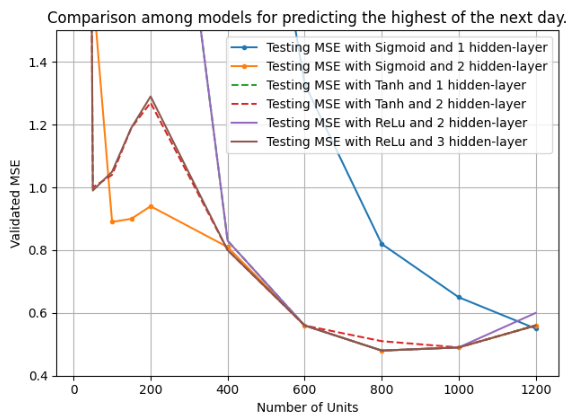
\includegraphics[height=5.5cm]{RNN_our1}
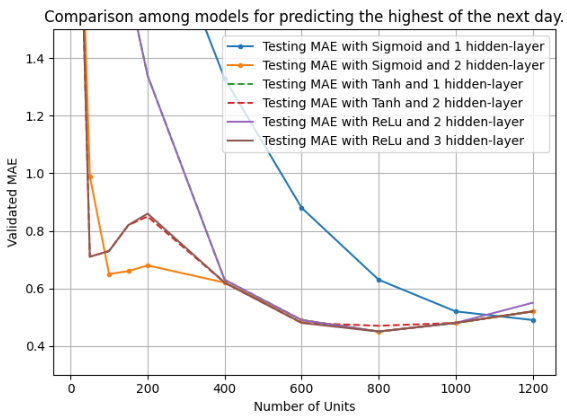
\includegraphics[height=5.5cm]{RNN_our2}
\end{figure}

\begin{figure}[H]
\label{fig:RNN Comparison for lowest}
\centering
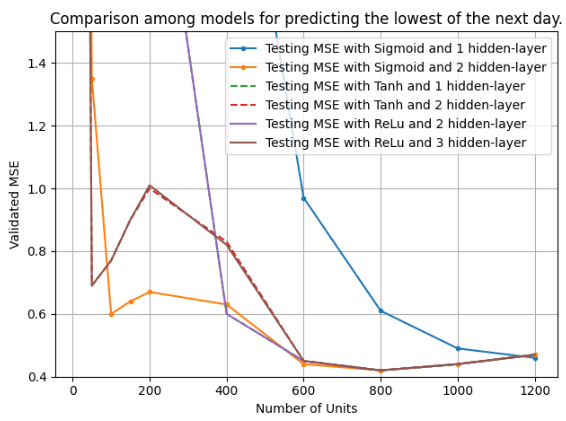
\includegraphics[height=5.5cm]{RNN_our5}
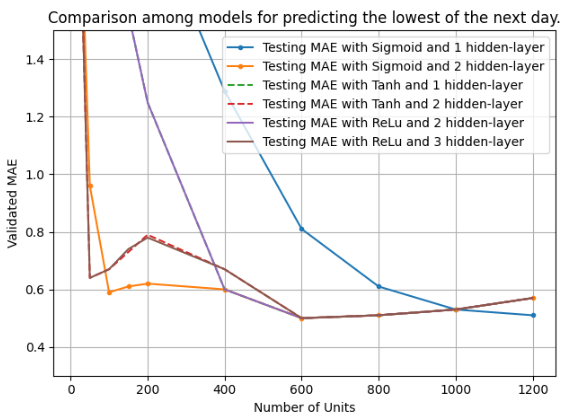
\includegraphics[height=5.5cm]{RNN_our6}
\caption{Comparison between all validated MSE (left) and MAE (right) when predicting the highest (top) and lowest (bottom) prices of the next day.}
\end{figure}\\

The activation function in which the best testing MSE and MAE scores converged to their minimum was Tanh. Besides, Tanh got the lowest scores with the lowest number of hidden-layers (1) and units (800), confirming to be the most promising and efficient model among the others. Therefore, the summary of parameters for this best model is: \\

\begin{table}[H]
\centering
\resizebox{\textwidth}{0.7cm}{
\begin{tabular}{ |c|c|c|c|c|c|c|c|c| }
\hline
\textbf{Target} & \textbf{Act.Funct.} & \textbf{H-Layers} & \textbf{Units} & \textbf{Epochs} & \textbf{Mini-batch} & \textbf{Loss-Funct.} & \textbf{Test MSE} & \textbf{Test MAE}\\
\hline
\textbf{Highest} & Tanh & 1 & 800 & 50 & 1 & MSE & 0.48 & 0.45\\
\textbf{Lowest} & Tanh & 1 & 800 & 50 & 1 & MSE & 0.42 & 0.51\\
\hline
\end{tabular}}
\label{table:Tanh, 1, 800, 50, 1, MSE}
\caption{Summary of parameters for our best model.}
\end{table}\\

It would be interesting to visualize the \textit{Train x Test} plots in order to analyse the bias and variance of the learning process:\\

\begin{figure}[H]
\label{fig:RNN train vs test for highest}
\centering
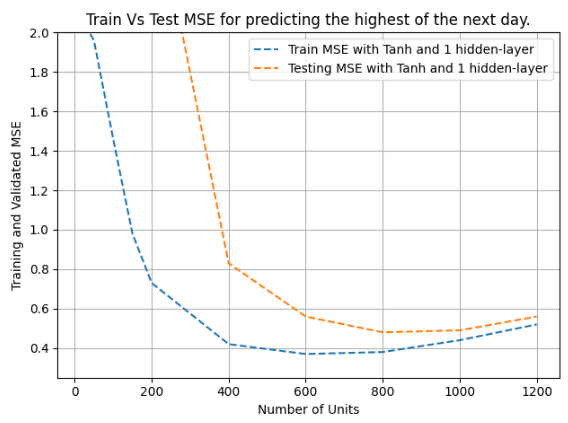
\includegraphics[height=5.5cm]{RNN_our3}
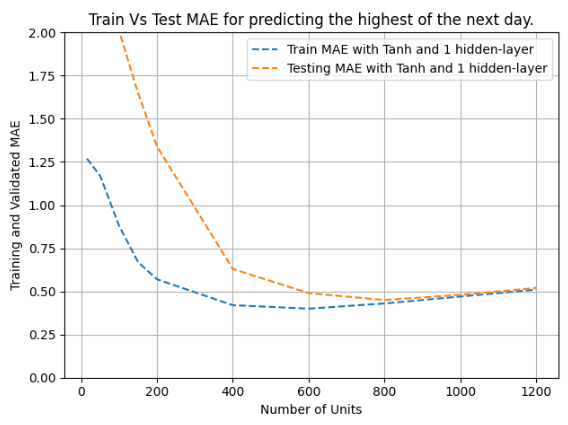
\includegraphics[height=5.5cm]{RNN_our4}
\end{figure}

\begin{figure}[H]
\label{fig:RNN train vs test for lowest}
\centering
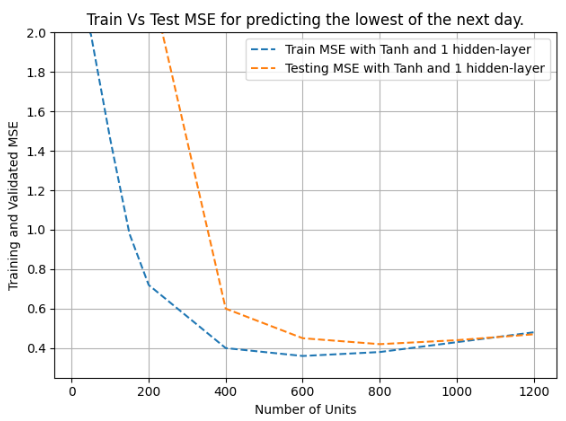
\includegraphics[height=5.5cm]{RNN_our7}
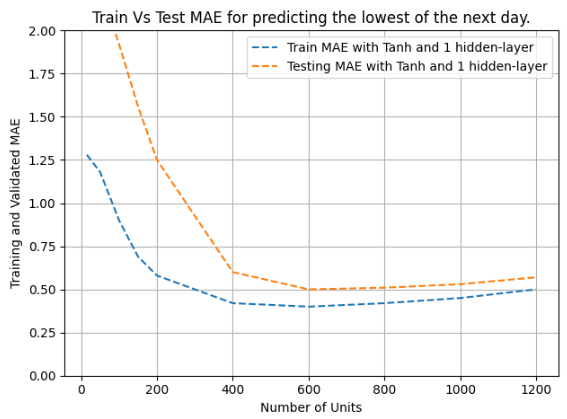
\includegraphics[height=5.5cm]{RNN_our8}
\caption{Train Vs Test MSE (left) and MAE (right) plots for the most promising and efficient model when predicting the highest (top) lowest (bottom) prices of the next day.}
\end{figure}

As expected, as the number of units increases, the metrics become more reliable until a certain point and then worsen again. We can visualize the same pattern in all plots, where the biases are very high for units before 200. As long the units grow around 800, it seems to reach the optimal point with very low biases and variance. After 800 units, we can notice that the metrics worsen, manifesting apparent over-fitting of the model, thus increasing the biases and variances.\\

Next, we need to check if the number of epochs can improve the model's metrics or efficiency. For that, we run a combination of epochs as a function of the optimized parameters:

\begin{table}[H]
\centering
\begin{tabular}{ |c|c|c|c|c|c| }
\hline
\textbf{Target} & \textbf{Epochs} & \textbf{Train MSE} & \textbf{Test MSE} & \textbf{Train MAE} & \textbf{Test MAE}\\
\hline
\rowcolor{lightgray} \textbf{Highest} & \textbf{10} & \textbf{0.3884} &	\textbf{0.4856} &	\textbf{0.4364} &	\textbf{0.4559}\\
Highest & 30 & 0.3884 &	0.4856 &	0.4364 &	0.4559\\
Highest & 50 & 0.3884 &	0.4856 &	0.4364 &	0.4559\\
Highest & 80 & 0.3884 &	0.4856 &	0.4364 &	0.4559\\
\hline
\rowcolor{lightgray} \textbf{Highest} & \textbf{10} & \textbf{0.3808} &	\textbf{0.4278} &	\textbf{0.4284} &	\textbf{0.5114}\\
Lowest & 30 & 0.3808 &	0.4278 &	0.4284 &	0.5114\\
Lowest & 50 & 0.3808 &	0.4278 &	0.4284 &	0.5114\\
Lowest & 80 & 0.3808 &	0.4278 &	0.4284 &	0.5114\\
\hline
\end{tabular}
\label{table:Results for RNN, Tanh, High, Epoch}
\caption{RNN model with parameters' combinations for predicting the next day's highest/lowest prices as a function of epochs.}
\end{table}

Remark that the metrics are precisely the same for 10, 30, 50, or 80 epochs, confirming that the SimpleRNN model converged to its minimum at ten epochs or before. Hence, we have improved our model's efficiency by decreasing from 50 to 10 epochs in the training process, and the final summary of parameters for our best model is:

\begin{table}[H]
\centering
\resizebox{\textwidth}{0.7cm}{
\begin{tabular}{ |c|c|c|c|c|c|c|c|c| }
\hline
\textbf{Target} & \textbf{Act.Funct.} & \textbf{H-Layers} & \textbf{Units} & \textbf{Epochs} & \textbf{Mini-batch} & \textbf{Loss-Funct.} & \textbf{Test MSE} & \textbf{Test MAE}\\
\hline
\textbf{Highest} & Tanh & 1 & 800 & 10 & 1 & MSE & 0.48 & 0.45\\
\textbf{Lowest} & Tanh & 1 & 800 & 10 & 1 & MSE & 0.42 & 0.51\\
\hline
\end{tabular}}
\label{table:Final, Tanh, 1, 800, 50, 1, MSE}
\caption{Final summary of parameters for our best model.}
\end{table}

\subsection{Applying the predictions to an algorithm trading strategy}
\label{chap:Applying the predictions to an algorithm trading strategy}


